\section{Ecossistema de software}

% ecossistema pode estar organizado em relacões de benefício mútuo

Ecossistema de software é definido, segundo \citeonline{manikas2013software},
como a interação entre diversos atores numa plataforma tecnológica comum
resultando em novas soluções de softwares ou novos serviços. Cada ator neste
sistema é motivado por um conjunto de interesses e conectam-se entre si e ao
próprio sistema numa relação simbiótica, fazendo a plataforma tecnológica
evoluir enquanto permite o envolvimento e contribuição de novos e diferentes
atores.

%software ecosystems.
%It is clear that the term was coined to reflect the organization of
%software vendors, third-party developers, suppliers, and users

%The term ecosystem usually refers to the operation of the system
%as a whole [1]. However, each individual plays an important role
%in the overall stability and sustainability of an ecosystem.

%Just like in natural ecosystems, software ecosystems need a conti-
%cont
%nuous input of energy in the form of new development or main-
%mai
%tenance of the ecosystem.

%\cite{dhungana2010software}

Nesta relação os atores são beneficiados de formas diferentes dependendo da
natureza do ecossistema, num ambiente comercial, por exemplo, os atores ganham
receita financeira diretamente (salário, prêmios, etc), enquanto num sistema
não-comercial os atores estão motivados por questões não-monetários (fama,
conhecimento, ideologia, etc).

De uma forma ou de outra, todos são beneficiados, os atores e o próprio
ecossistema, os atores recebem mais (ou melhores) benefícios com o crescimento
do ecossistema, o ecossistema oferece cada vez mais (ou melhores) benefícios
com as atividades dos seus atores, resultando numa relação de benefício
mútuo.

Este modelo geral de funcionamento do ecossistema de software pode variar a
depender do contexto em que se insere, o ecosistema de software acadêmico por
exemplo possui a particularidade de estar inserido no sistema de reputação
científica de alguma forma.

%possibilita esse tipo relação simbiótica
%apesar de não determinar que todo ecossistema aproveite tal benefício.
%
%Adicionalmente as relacões entre os atores do ecosistema como um todo
%são de mútuo interesse (mutualismo):
%
%O relacionamento entre os atores em um ecossistema de software, por outro lado,
%são caracterizados pela alto espectro de relacionamentos simbioticos.
%
%Dependendo dos atores e suas atividades, dois atores podem ter benefícios
%mútuos (mutualismo), estar em competição direta (competition/antagonism),
%estarem não afetados (neutralism) ou um não afetado enquanto o outro é
%beneficiado (amensalism) ou prejudicado (parasitism) por seu relacionamento

\section{Ecossistema de software acadêmico}

O ecossistema de software acadêmico possui a particularidade de estar inserido
num contexto que se relaciona com a economia de reputação científica,
especialmente com o sistema de publicação, sendo influenciado e influenciando
diretamente o impacto causado pelas suas publicações e pelo seu sistema de crédito
acadêmico.

% (5) Tools in mining software repositories \cite{chaturvedi2013tools}
% Faz uma revisão dos papers submetidos ao MSR desde 2007 até 2013 (?) e
% identifica data sets, ferramentas e técnicas utilizadas pelos autores, mais
% da metade dos papers usam ou criam ferramentas, categoriza as ferramentas em
% ferramentas novas, ferramentas tradicionais, protótipos e scripts para
% mineração de dados

\citeonline{howison2015understanding} criou um framework para pensar e refletir
sobre o processo de produção de softwares na ciência, e identificou quatro
papéis envolvidos no ecossistema de softwares acadêmicos, cientistas usuários
finais, produtores e distribuidores de software, administradores de
infraestrutura e pesquisadores preocupados com o funcionamento do ecossistema
como um todo.

%Unlike other technologies supporting science, software can
%be copied and distributed at essentially no cost, potentially
%opening the door to unprecedented levels of sharing and col-
%laborative innovation. \cite{howison2011scientific}
%
%While some of these seem relatively unproblematic, such as commercial
%production in fields with immediately valuable applications, others appear
%problematic. In particular we highlighted the potentially pernicious
%implications of the academic credit production system for collaboration and
%maintenance.

\subsection{Cientistas usuários finais}

Pesquisadores de todos os domínio da ciência ocupam um papel chave no
ecossistema de software acadêmico, em seus processos de investigação e
experimentação fazem uso de artefatos de software para coletar, gerenciar,
transformar, analisar, modelar e visualizar os seus dados, sempre com o
objetivo final de publicar os seus resultados na literatura acadêmica.

Os cientistas estão preocupados com a disponibilidade, qualidade e usabilidade
destes artefatos de software e também com a capacidade de continuar úteis
podendo ser utilizados em conjunto com outros softwares. Estão interessados
também em saber o que outros cientistas usam em suas pesquisas, softwares com
alta adoção no domínio em que estão inseridos costumam manter os pesquisadores
mais livres e com maior foco em suas próprias pesquisas.

Uma alta adoção costuma ser sinal de uma boa qualidade de software, além
garantir que o grupo de pesquisa, estudantes e colaboradores consigam encontrar
mais facilmente o software e também obter ajuda entre os seus pares para
resolver questões sobre o uso do softare, simplifica também o trabalho dos
revisores pois encontrarão as mesmas facilidades no uso.

\subsection{Produtor e distribuidor de software acadêmico}

Este papel pode ser desempenhado por indivíduos ou times, softwares acadêmicos
costumam ser desenvolvidos em colaborações próximas entre cientistas da
computação e cientistas de outras áreas, usualmente sendo o cientista da
computação responsável por desenvolver algoritmos que refletem as pesquisas
destes outros pesquisadores.

Um desafio comum enfrentado pelo cientista da computação é abstrair os
problemas e implementar soluções que podem ser adotadas por outros cientistas,
especialmente em outros domínios. Alguns softwares são desenvolvidos e muitas
vezes ficam confinados em seus laboratórios ou grupos, mas eventualmente são
compartilhados e potencialmente amplamente adotados, tornando o cientista autor
do software e da pesquisa parte do ecossistema do software (Van de Geijin 1997).

Estes atores preocupam-se com o impacto cientifico tanto em termos de numero
quando de tipos de usuários que seu software atinge, e como seus softwares
contribuem para a ciencia que outros estão realizando.

Alguns projetos são gerenciados no estilo de código aberto, e tem atraido com
sucesso contribuições de muitos cientistas, incluindo uma calda longa de
contriuição que tem feito pequenas mas substanciais contribuições.

\subsection{Provedor de infraestrutura}

O provedor de infraestrutura é aquele que provê um cojunto de softwares aos
cientistas usuários finais, para que dêem apoio em seus trabalhos de pesquisa.
Este conjunto de softwares podem estar disponíveis para o usuário final fazer
download eu seus computadores pessoais ou podem ser serviços de
ciberinfraestrutura de software hospedados em centros de supercomputação
usando provedores de computação em nuvem.

Do ponto de vista de ecossistema ambos os tipos de distribuição estão
interessados nas mesmas questões, quem usa ou não usa, qual versão é utilizada,
com qual frequencia atualizam, etc.

\subsection{Pesquisador}

Este último papel chamado aqui de pesquisador num sentido amplo da palavra,
refere-se à qualquer um preocupado sobre o funcionamento do próprio ecossistema
e sobre o sua contribuição para a ciência como um todo, costuma ser
desempenhado por agencias de financiamento, mas abrange qualquer cientista
preocupado com os seu trabalho individual ou do seu campo de pesquisa.

As preocupações rondam ao redor de questões sobre a operação do ecossistema como
um sistema que consome recursos (tempo, dinheiro e atenção) e afeta a conduta da
ciência, tanto no geral como em campos específicos, complementado pelo interesse
de saber como o comportamento desse sistema pode ser influenciado.

%Junto com estas questões estão as questões de como influenciar o ecossistema,
%incluindo questões de pontos de inflexão que levam ao uso coalescente, bem como
%a intervenções políticas diretas incentivando o uso de componentes específicos.

\section{Modelo de processo de softwares na ciência}

% recurso, uso e impacto

%Computer systems research spans sub-disciplines that in-
%clude embedded and real-time systems, compilers, network-
%ing, and operating systems. Our contention is that a number
%of structural factors inhibit quality research. We highlight
%some of the factors we have encountered in our work and ob-
%served in published papers and propose solutions that could
%both increase the productivity of researchers and the quality
%of their output \cite{Vitek2011}.

Estes atores participam do ecossistema dentro de seus próprios interesses, mas
sempre causando um impacto de volta no sistema, os cientistas usuários finais
(direta ou indiretamente) usam softwares acadêmicos para fazer ciência,
resultando em impacto científico, este impacto científico então justifica
investimentos de novos recursos, que faz o ecossistema crescer a partir da
evolução destes softwares ou a partir da produção de novos softwares.

\begin{figure}[h]
  \center
  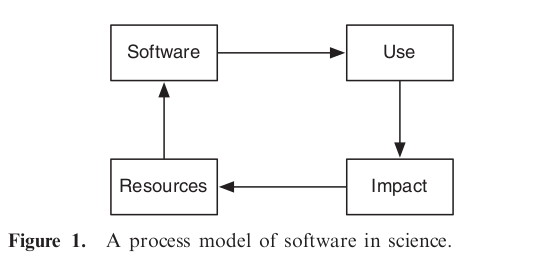
\includegraphics[scale=0.5]{imagens/process-model-scientific-software.png}
  \caption{A process model of software in science \cite{howison2015understanding}}
  \label{process-model-scientific-software}
\end{figure}

A Figura \ref{process-model-scientific-software} apresenta um diagrama deste
modelo de processo de softwares na ciência, este modelo é detalhado à seguir,
cada ator atua nos softwares, recursos, uso, impacto científico, detalhados à
seguir.

%seja para fins de planejamento ou reflexão
%seja como retrospectiva para avaliar investimentos realizados.
%
%Recursos são devotados para a produção de software acadêmico. Usuários finais
%cientistas (diretamente ou indiretamente) usam softwares acadêmicos para fazer
%ciência, resultando em impacto científico. Impacto científico então justifica
%investimentos e recursos, seja de forma antecipada para fins de planejamento,
%seja como retrospectiva para avaliar investimentos realizados.

\subsection{Software}

Software acadêmico ({\it academic software}) é todo software usado para
coletar, processar ou analisar resultados de pesquisas com intenção de ser
publicados na literatura academica (seja num jornal, revista, conferência,
monografia, livro ou tese), podem ser desde protótipos escritos pelos próprios
cientistas, até mesmo produtos completos desenvolvidos profissionalmente
\cite{allen2017engineering}.

Podem ser encontrados na literatura acadêmica com outros nomes,
{\it research tool} \cite{Portillo12},
{\it research-originated software} \cite{Kon2011},
{\it research software} \cite{hettrick_2014_14809} ou
{\it scientific software} \cite{segal2008developing},
cinco modelos de produção de software na ciência, distinguidos principalmente
pela motivação principal: (1) ganho monetário direto (comercial software,
employed software developers), (2) reputação acadêmica (incidental software,
dirigido pela necessidade científica direta), (3) prática de software paralela
(scientific needed enhanced by publishing 'software papers' alongside domain research),
(4) um software de uma subárea de pesquisa (reputação direta pelo trabalho do software),
(5) híbridos como licença-dual e 'software work' dentro de grandes colaborações
(software como uma contribuição científica direta).

\subsection{Recursos}

Os recursos investidos na produção destes softwares vem de diversas fontes,
incluem ganhos monetários diretos, recursos alocados em projetos, colaboração
entre laboratórios de pesquisa, e grande parte do ``tempo livre'' dos
pesquisadores em busca de soluções em suas pesquisas, este ``tempo livre''
perpassa por financiamentos diversos, carreira individual do cientista,
estudantes de graduação, prêmios, etc.

Independente da origem dos recursos o desenvolvimento de softwares acadêmicos
possui a particularidade de ser desenvolvido em sua grande maioria pelos
próprios cientistas \cite{segal2008developing, hettrick_2014_14809,
momcheva2015software}.

\subsection{Uso}

% ... software é distribuido, utilizado e dá suporte à ciencia, gerando impacto ...

Estes artefatos de software são usados ativamente em diversos campos de pesquisa, como
matemática, biologia, física de partículas, astronomia, medicina e direito,
eles resolvem problemas comuns do cotidiano de pelo menos metade dos
pesquisadores de todas as áreas, desde grupos trabalhando exclusivamente com
problemas computacionais até grupos em laboratórios tradicionais ou em campo
\cite{wilson2014best}.

Os cientistas usuários finais mencionam tais softwares em suas publicações,
seja através de citação formal, informal, ou qualquer outro tipo de menção ao
software em suas pesquisas, estas citações ou menções fazem parte da economia
de reputação científica e causam impacto científico.

\subsection{Impacto científico}

% ... impacto científico justifica e potencialmente gera mais recurso ...
% \cite{katz2014transitive}

Ao longo da história, a citação formal tem sido utilizada para garantir
autenticação e autoridade, em vez de dar crédito e promover reconhecimento, na
história ocidental a citação aparece no final dos anos 1500, no início dos anos
1700 surge também no sistema legal, o ``copyright'' como reconhecendo aos
direitos autorais também surge nesse período, 1710.

A autoria das publicações tem sido realmente usado para reconhecer os autores e
contribuidores de um certo estudo, por exemplo, nos casos em que vários grupos
reivindicam crédito pelo mesmo avanço, ``backward citing'' tem sido utilizado
para verificar como as maiores comunidades de pesquisa atribuem crédito,
``forward citing'' também tem sido usada em casos onde se quer entender como
uma idéia foi usada após o seu surgimento ou publicação.

Conhecimento novo é claramente construído a partir do conhecimento passado.
Tradicionalmente, um autor cita um artigo anterior adicionando uma referência
ao autor, título, local de publicação, etc. No entanto, esse conceito não
funciona bem para produtos digitais como o software, que muitas vezes depende
de outros softwares, fragmentos de código, e algoritmos.

Este debate tem sido realizado a bastante tempo entre as diversas áreas da
bibliometria, cienciometria, altmetria e áreas similares, o fator de impacto
por exemplo proposto em 1955 apesar de continuar contribuindo para a ciência se
mostra muitas vezes utilizado da forma errada e mostra as deficiências de lidar
bem com produtos digitais gerados durante pesquisas.

%historia da citacao na ciencia, como isso promove o avanço, problemas para
%citacao em artefatos digitais, solucao para identificador unico de autores de
%artigos, orcid.org resolve este problema, o mesmo para identificar artefatos
%digitais é o doi.org

%No entanto tem se percebido que o ecossistema de software acadêmico tem perdido
%oportunidade de colaboração visto que estão inseridos neste contexto ....
%competição, muitos softwares utilizados em pesquisas não são mencionados
%pelos seus autores causando impacto negativo em sua visibilidade, reconhecimento e
%consequentemente ...  \cite{howison2016software}.
%
%A comunidade tem refletido sobre os problemas relacionados ao
%desenvolvimento, promoção e sustentabilidade desses softwares, e o
%impacto que tais problemas causam no meio científico \cite{allen2017engineering}. Esta
%reflexão tem mostrado, por exemplo, que muitos estudos em engenharia de
%software sofrem de dificuldades de repetição \cite{Tang2016}, e apontam
%problemas específicos relacionados à manutenabilidade e a sustentabilidade
%técnica dos softwares acadêmicos.

\section{Desenvolvimento, reconhecimento e sustentabilidade de software acadêmico}

% problemas identificados no ecossistema de software acadêmico

Um estudo sobre ecossistema de software acadêmico percebeu através dos relatos
de grande parte dos colaboradores participantes do estudo que os projetos de software
acadêmicos desenvolvidos na própria academia sofrem de {\it ``dysfunctional
chaotic churn''}, ou seja, a existência de muitos projetos, com poucos
usuários, com ciclos de vida curtos, que terminam em paralelo ao financiamento
inicial, comunidades desconectadas e paralelas, incompatibilidades entre
projetos, e tentativas aparentemente não coordenadas de ``reiniciar'' tudo
({\it re-boots}) \cite{howison2015understanding}.

%Este cenário, além de desacelerar o progresso geral da ciência gerando
%retrabalho, faz surgir questionamentos sobre as conclusões dessas pesquisas,
%especialmente quando grande parte dos pesquisadores não sabem o quão confiável
%seus softwares são.

Apesar de não haver evidências a respeito deste problema de forma tão abrangente,
sabe-se que parte dos problemas são realmente fato, por exemplo,
o {\it Dagstuhl Perspective Workshop}, evento organizado por um grupo de
pesquisadores sêniores de renome internacional, realizado anualmente na
universidade de Dagstuhl\footnote{\url{http://www.dagstuhl.de}} com o objetivo
refletir sobre o estado da ciência da computação explorando tópicos novos e
emergentes, em sua mais recente edição o workshop debateu sobre software
acadêmico e os problemas comuns em seu desenvolvimento, reconhecimento e
sustentabilidade \cite{allen2017engineering}.

\subsection{Desenvolvimento}

O desenvolvimento de software acadêmico ocorre em grande parte dentro da
própria academia, estudos mostram que pelo menos metade dos cientistas desenvolvem
seus próprios softwares, ao menos pacialmente, em domínios específicos este
número pode ser bem maior, na astronomia, por exemplo, estudos mostram que este
número pode chegar a 90\% \cite{hettrick_2014_14809, momcheva2015software}.

% do reino unido mostrou que 56\%

A grande participação dos cientistas no desenvolvimento destes artefatos de
software costuma ser um reflexo do tipo de conhecimento necessário ao se
desenvolver tais artefatos de software, pode ser necessário entender como o DNA
genômico se transforma em cristais de proteína, ou os meandros da dinâmica dos
fluidos, ou como resolver 20 equações diferenciais parciais simultâneas
\cite{segal2008developing}.

Desenvolvimento de software, exige algum conhecimento sobre o domínio, software
acadêmico não é diferente, mas esta grande participação dos cientistas no
desenvolvimento de software acadêmico começa a se tornar uma preocupação à
medida que a maior parte não possui treinamento algum sobre como escrever
softwares de forma eficiente, muitos não testam ou documentam os seus
softwares, faltam práticas básicas de desenvolvimento, como escrever código
legível, revisão de código, controle de versão, testes unitários, entre outros
\cite{wilson2017good}.

Ocasionando sérios erros computacionais em conclusões centrais da literatura
acadêmica, gerando retrabalho para retratar tais erros nas mais diversas áreas
da ciência \cite{Merali2010Computational}. Dados são perdidos, análises levam
mais tempo que o necessário e os pesquisadores não conseguem a eficiência que
poderiam ter ao trabalhar com softwares acadêmicos \cite{wilson2017good}.
Causando um impacto negativo na visibilidade dos softwares acadêmicos
\cite{howison2013, katz2014transitive} e na capacidade de serem encontrados e
compartilhados.

%, e faz
%surgir questionamentos sobre sua qualidade, não apenas técnica, mas também a
%capacidade de ser encontrado, compartilhado e co-desenvolvido, qualidades
%importantes para a evolução do próprio software, mas também extremamente úteis
%para o uso eficiente dos limitados recursos da ciência \cite{howison2013,
%katz2014transitive}.

\subsection{Reconhecimento}

% Visibilidade

Apesar do crescimento no uso de software e na consequente dependência entre
cientistas de todos os campos, tornando o software acadêmico parte integral da
prática científica, apesar do apelo da comunidade científica para que o
software acadêmico seja tratado como cidadão de primeira classe, estudos tem
mostrado que muitas pesquisas não mencionam sequer o uso de software acadêmico
em suas publicações mesmo tendo feito uso de tais artefatos
\cite{momcheva2015software} \cite{howison2016software}.

Isto tem prejudicado a visibilidade do software acadêmico causando impacto
negativo em seu ecossistema, um software invisível é frequentemente excluído de
revisões por pares, uma atividade que costuma contribuir para a qualidade geral
do trabalho publicado, além disso, o
impacto negativo na visibilidade do software acadêmico faz surgir uma
série de questionamentos sobre a sua qualidade e também sobre a
capacidade de ser encontrado, compartilhado e co-desenvolvido
\cite{howison2013, katz2014transitive} \cite{howison2016software}.

Um software acadêmico em bom funcionamento devem atingir não apenas os
objetivos de entendimento e transparencia, mas também os objetivos voltados
para replicação \cite{Stodden2010}, seja logo após sua publicação, seja daqui
a 10 ou 50 anos.


%apesar de não existir um consenso sobre como citar
%artefatos digitais e outros tipos de produtos científicos,
%existem inúmeras sugestões de formalização e inúmeras práticas
%formais e informais.

%citações formais facilitam e promovem o avanço
%da ciência, mesmo diante da falta de um padrão para citar artefatos digitais
%\cite{allen2014credit}.

%Um estudo recente com 90 artigos de diversas áreas da biologia, selecionados
%aleatoriamente entre publicações usando softwares como método, mostrou que
%apenas 59 mencionavam o uso de softwares de alguma forma, os demais 31 artigos,
%apesar de usar software acadêmico, não mencionavam nada a respeito
%\cite{howison2016software}, apenas entre 31\% e 43\% das menções aos softwares
%acadêmicos envolvem citação formal.

%Não existe ainda amadurecimento suficiente sobre como citar softwares e
%outros artefatos digitais em pesquisas científicas, não temos um padrão de como fazê-lo,
%cada autor cita à sua maneira, muitas vezes ao longo do texto, outras em seções
%específicas sobre a implementação do software, nem semprem informam onde
%encontrar uma cópia do software, ou ainda nem sobre o modelo em que o software
%é distribuído, ou se é de alguma forma distribuído ao público.

%Entre os softwares acadêmicos desenvolvidos por cientistas como apoio em suas
%pesquisas, não é raro que pesquisadores deixem de disponibilizar estes artefatos,
%assim como outros desdobramentos da pesquisa, como dados e outros. Ou ainda,
%mesmo disponibilizando tais artefatos em locais de público acesso, com o tempo,
%tais locais se tornam indisponíveis inviabilizando a obtenção de tais
%artefatos.

\subsection{Sustentabilidade}

O desenvolvimento de software sustentável tem sido identificado como um desafio
chave no campo da ciência e da engenharia computacional, se sustentabilidade
não for levada em consideração em projetos de software, não importa qual o
domínio ou qual o propósito do software, perde-se a oportunidade de causar
mudanças positivas no planeta e na sociedade.

Apesar de sustentabilidade ser um conceito complexo e com mútiplas dimensões,
levando a debates profundos, o conceito geral é bastante simples e refe-se à
capacidade de perdurar e de continuar sendo suportado ao longo do tempo, isto
implica na qualidade de longevidade e manunetabilidade do software
\cite{venters2014software}.

Software sustentável é aquele que continua a estar disponível no futuro, em
novas plataformas, atendendo continuamente às novas necessidades do ambiente
... adequada evolução frente as condições do ambiente em constante mudança
\cite{allen2017engineering}.

Estudo mostra o decaimento das URLs ao longo do tempo, fundamenta o assunto,
mostra grafico com o caimento ao longo dos anos em publicações da
bioinformática, grafico muito bom cruzando e decaimento e tendencia com os
passar do tempo \cite{wren2017use}.

%Diversas iniciativas tem sido tomadas em relação a garantir a longevidade dos
%artefatos,

O {\it Journal of the American Statistical Association (JASA)} tem insistido na
necessiade de estarem disponíveis código e dados durante a revisão dos
manuscritos \cite{baker2016scientists}, Agências de financiamento como o {\it
US National Science Foundation} estão começando a reconhecer produtos de
pesquisa, como software, assim como fazem com as publicações, isto reconhece as
contribuições ao softwares assim como primeiro produto de pesquisa.

%este artigo \cite{howison2016software} faz exatamento o mesmo estudo que estou fazendo!
%A well-functioning system
%would assist not only the goals of understanding and trans-
%parency, but also the goals of aiding replication (Stodden
%et al., 2010), complementing the availability of publications
%such that “the second researcher will receive all the benefits
%of the first researcher’s hard work” (King, 1995, p. 445).

Isto visa especialmente garantir a longevidade dos artefatos e proporcionar que
um segundo pesquisador receba todos os benefícios do trabalho duro do primeiro
pesquisador \citeonline{king1995replication}, já que tanto a ciência quanto a
engenharia dependem de resultados incrementais para sua evolução. No terceiro
compromisso, relacionado ao conceito {\it desenvolvimento}, o Dagstuhl
Manifesto enfatiza a necessidade de medir a qualidade e a sustentabilidade dos
softwares científicos, tanto a priori quanto a posteriori.

\subsubsection{Manutenabilidade}

% falar de manutenabilidade como um eixo dentro de sustentabilidade técnica

A qualidade dos softwares acadêmicos tem sido questionada,
a maioria também não sabe o quão confiável seu software é \cite{Merali2010Computational},
muitos estão em estado inicial de desenvolvimento \cite{marshall2013tools},
poucas foram testados fora do contexto onde foi desenvolvido \cite{Portillo12}.

%Cita um mapeamento sistemático com objetivo de encontrar ferramentas de
%comunicação e coordenação para suporte a times altamente distribuidos
%gograficamente, encontrou 132 ferramentas, para uso em projetos de software
%global. A maioria destas ferramentas foram desenvolvidas em centros de
%pesquisas, e apenas uma pequena porcentagem (18.9\%) foram testados fora do
%seu contexto onde foi desenvolvido \cite{Portillo12}.
%
%Cita um mapeamento feito sobre estudos que criam ferramentas para apoio a
%revisão sistemática no domínio de SE, 14 estudos foram selecionados, ao final
%apenas 8 tinham proposta de ferramentas, ao final conclui que as ferramentas
%encontradas estão em estado inicial de desenvolvimento \cite{marshall2013tools}.

A adoção e uso de softwares acadêmicos está relacionada, entre outros fatores,
também à sua qualidade, portanto é impoprtante medir e coletar sua qualidade de
alguma forma, qualidade é um vasto assunto, um dos problemas comuns enfrentado
pelos pesquisadores que desenvolvem tais softwares é a manutenabilidade
\cite{Prlic2012}.

Apesar de nem sempre ser possível, ou viável, ter tudo dentro de padrões
estritos, é preciso estar consciente das boas práticas ao produzir e utilizar
softwares acadêmicos, tanto para melhorar a própria abordagem quanto para
revisar outros trabalhos \cite{wilson2014best}.

Mas não só de qualidade interna vive o software, a capacidade de estar disponível, seja
de forma comercial, gratuita ou livre, documentação, instruções de uso, etc.

%Além da aplicação, estes softwares variam também no papel que ocupam em suas
%pesquisas, alguns fazem parte dos resultados da pesquisa, como por exemplo,
%propostas de novos algoritmos ou técnicas de produção, outros são utilizados
%como parte do método de pesquisa, como coleta ou análise de dados, sendo que
%estes papeis não são excludentes.
%
%estes costumam ser citados pelos seus autores como uma das contribuições do
%estudo, seja principal ou secundária, 
%Esses softwares podem, de fato, ser um software de simulação complexo desenvolvido
%e executado em um computador de alto desempenho, mas também pode ser um
%software desenvolvido em um PC para incorporação em instrumentos; para
%manipular, analisar ou visualizar dados; ou para orquestrar fluxos de trabalho.
%
%e à medida
%que percebe-se que os softwares estão se tornando parte integrante dos
%processos, ferramentas e produção científicas, torna-se necessário e urgente
%discutir o seu desenvolvimento, visibilidade, qualidade e sustentabilidade.
%
% ecossistema pode estar organizado em relacões de benefício mútuo
% 
% mostrar os beneficios da ciencia aberta, ciberinfraestrutura, etc
% * (favorecendo a ciencia e tornando a vida mais feliz para todos)
% 
% ecossistema de software acadêmico está inserido num contexto de competição
% 
% mostrar os problemas para a ciência como um todo
% * causando problemas para o progresso de ciência, dados perdidos, etc, retrabalho
%   dificuldade de reprodução, etc...


%Estes são alguns problemas relacionados aos softwares acadêmicos, muitos são
%resultado de baixos orçamentos, limitação de tempo e alta rotatividade entre os
%grupos de pesquisa, outros são, possivelmente, ocasionados por questões
%culturais \cite{niemeyer2017open}, como, por exemplo, a tímida adoção de
%práticas da ciência aberta entre pesquisadores. Compreender os reais motivos
%por trás destes problemas seria, naturalmente, o passo essencial para solucioná-los,
%apesar disso, antes mesmo de resolver tais questões é
%fundamental compreender os impactos que eles causam na comunidade de pesquisa.

%, não apenas técnica, mas também a
%capacidade de ser encontrado, compartilhado e co-desenvolvido, qualidades
%importantes para a evolução do próprio software, mas também extremamente útil
%para um uso eficiente dos limitados recursos da ciência \cite{howison2013,
%katz2014transitive}.
%
%contradizendo as boas
%práticas de qualquer projeto experimental, de ter {\it laboratory
%notebooks}\footnote{\url{https://en.wikipedia.org/wiki/Lab_notebook}}, dados
%organizados, passos documentados, e projeto estruturado para reprodutibilidade.
%
%softwares acadêmicos, assim
%como qualquer outro aparato experimental, são tão importantes para a ciência
%quanto são os telescópios ou tubos de ensaio \cite{wilson2014best}.
%
%Cientistas gastam mais tempo hoje utilizando e desenvolvendo softwares do que
%gastavam no passado.
%
%Software is a critical part of modern research and yet there is little support across the
%scholarly ecosystem for its acknowledgement and citation. Inspired by the activities
%of the FORCE11 working group focused on data citation, this document
%summarizes the recommendations of the FORCE11 Software Citation Working
%Group and its activities between June 2015 and April 2016. Based on a review of
%existing community practices, the goal of the working group was to produce a
%consolidated set of citation principles that may encourage broad adoption of a
%consistent policy for software citation across disciplines and venues. Our work is
%presented here as a set of software citation principles, a discussion of the motivations
%for developing the principles, reviews of existing community practice, and a
%discussion of the requirements these principles would place upon different
%stakeholders. Working examples and possible technical solutions for how these
%principles can be implemented will be discussed in a separate paper.
%\cite{smith2016software}

%Isto se torna ainda mais difícil visto que frequentemente os pesquisadores
%deixam de publicar o código dos seus softwares acadêmicos argumentando que o
%código é ``ruim'' e isto irá gerar julgamentos negativos ao pesquisador
%\cite{allen2017engineering}.

%Improving academic software engineering projects: A comparative study of academic and industry projects
%(compara as praticas de desenvolvimento da industria e academia e sugere melhorias, 1998!)
%https://link.springer.com/article/10.1023%2FA%3A1018925902814?LI=true

% papel pesquisador no ecossistema de soft academico
%
%Essas preocupações gerais sugerem um conjunto de questões específicas, com foco
%em padrões globais e padrões emergentes dentro do ecossistema, incluindo: Quais
%recursos foram destinados à produção de software? Quantos usuários ou
%comunidades de usuários têm projetos? Quais são os impactos científicos desse
%uso? Os números de usuários crescem? Os projetos possuem recursos e habilidades
%suficientes para gerenciar seu crescimento? Quais projetos possuem
%funcionalidades sobrepostas? Há quanto tempo os pedaços de software e projetos
%persistem? Nós desconectamos as comunidades de usuários e desenvolvedores? São
%componentes específicos, ou camadas de componentes, faltam? Que código
%geralmente é usado em conjunto; são os projetos e as pessoas que produzem esses
%componentes se comunicando adequadamente? Como podemos sustentar o software
%crítico?
%
%Aqui há uma clara tensão entre um desejo de flexibilidade e liberdade, ligado
%às expectativas de inovação científica e desejos de estruturas de autoridade e
%controle de coordenação. As questões de influência incluem: como os programas
%de financiamento e quais os requisitos em suas chamadas, resultaram em software
%amplamente utilizado e impacto científico substancial? Quais são as
%características dos campos que alcançaram maior coalescência? Quais jornais e
%conferências têm políticas exemplares? Como o trabalho de software é visto
%dentro das práticas de contratação e avaliação, como os casos de posse?
%
%\cite{howison2015understanding}

%Ao longo da história, a citação formal foi para autenticação e autoridade, em
%vez de de crédito e reconhecimento ou atribuição. A  científico citação na
%história ocidental aparece no final dos anos 1500. No início dos anos 1700, a
%citação também aparece no sistema legal como método de compreensão dos
%precedentes \cite{katz2014transitive}.
%
%A ideia de direitos autorais como reconhecendo aos direitos dos seus autores
%também surge nesse tempo, 1710, talvez devido a uma lenta tendência social
%societária de reconhecer a propriedade intelectual, uma idéia que parece ter se
%desenvolvido ao lado da imprensa]. Observe que a autoria de papers é realmente
%usado para notar os autores reais do artigo quanto para notar os contribuidores
%do projeto.
%Para muitos desses, o
%identificador que deve ser citado - um "nome" que se refere a um produto único
%não é claro.
%
%Additionally, if a cited library depends
%on another library, the contribution of this second library
%is not captured. Citation of a dataset should perhaps give
%credit to the people who gathered the data, as well as
%those who curated it, but the paper author may not know
%or be able to find these details.

%Mas independente de como seja calculado o impacto científico de uma determinada
%pesquisa o impacto causado se reverte potencialmente em mais recursos que
%poderão ser reinvestidos no próprio ecossistema onde o software está inserido.

%%%%%%%%%%%%%%%

%Os compromissos expressados neste manifesto são agrupados em três conceitos gerais:
%(i) garantir que softwares científicos sejam {\it citados} apropriadamente;
%(ii) promover a {\it carreira} do engenheiro de software desenvolvedor de software científico; e
%(iii) medir a qualidade e sustentabilidade do software científico durante e após o seu {\it desenvolvimento}.

%um caminho apontado como solução é acreditar que software deve evoluir para plataformas compartilhadas,
%com componentes reusáveis tanto quanto possível, tanto para usuário final, quanto
%para produtores de componentes (papel) agregando peças particulares de software,
%crença de que o software deve evoluir em direção a uma plataforma
%compartilhada, com componentes que são reutilizados o mais amplamente possível,
%já que os usuários finais e os produtores de componentes se agrupam em torno de
%peças específicas de software.

%Science Code Manifesto \cite{barnes2013science}.
%Foco em código fonte escrito especificamente para processar dados de
%publicações, afirma que ``todo código fonte escrito especificamente para
%processar dados de uma publicação deve estar disponível para os revisores e
%leitores do paper''.

%O ecossistema de software acadêmico possui a particularidade de estar inserido
%num contexto de competição que se relaciona com a economia de reputação
%científica, em alguns pontos, como no mecanismo de crédito acadêmico às
%produções ser potencialmente problemático para a colaboração e manutenção.

%Sustentabilidade é um conceito sistêmico e precisa ser entendido em conjunto
%com suas diversar dimensões, 

%Sustentabilidade técnica diz respeito a longevidade dos softwares, ou seja, a
%capacidade de continuar disponível no futuro.

%Essa definição de sustentabilidade de software é encontrada em mais detalhes no
%{\it Karlskrona Manifesto} \cite{becker2014karlskrona}, um documento que alerta
%sobre os impactos que os sistemas e a tecnologia da informação causam no futuro
%do planeta, convida praticantes e pesquisadores de software a refletir sobre
%o tema sustentabilidade na área da ciência da computação.

%Sustentabilidade é um conceito guarda chuva composto de múltiplas dimensões, em
%sua dimensão técnica, chamada sustentabilidade técnica, temos a preocupação com
%a longevidade da informação, dos sistemas, e infraestrutura, e sua adequada
%evolução frente as condições do ambiente em constante mudança.

%Software ocupa
%um papel central nessa discussão, ele pode levar a crescentes consumo de
%recurso, crescimento da desigualdade social, e influenciar no ganho ou perda de
%auto-estima individual.
